\documentclass{beamer}
\usepackage{epstopdf}
\usepackage{adjustbox}
\usepackage{tikz}
\usepackage{arydshln} %Dotted lines for tables \hdashline \cdashline
\usepackage{import}
\usetikzlibrary{
	positioning				% Allows 5px above/below of x style positioning
	, arrows				% Allows <-, ->, <-> style arrows.
	, fit					% Allows fitting lines to shapes
	, decorations.pathreplacing	% Allows decoration that affect line paths.
	, backgrounds
	, shapes
	, shapes.multipart
	, calc
	, chains
}
\usepackage{todonotes}

\mode<presentation> {
	\usetheme{Malmoe}
	\usecolortheme{whale}
	\setbeamertemplate{footline}[page number]
	\setbeamertemplate{navigation symbols}{}
}

%----------------------------------------------------------------------------------------
%	TITLE PAGE
%----------------------------------------------------------------------------------------

\title[Short title]{Project NUClear}

\author{
	Trent Houliston \and Jake Woods \and Joshua Kearns \and Michael Burton
}

\institute[UoN]
{
	University of Newcastle \\ % Your institution for the title page
	\medskip
	\textit{\{Trent.Houliston, Jake.F.Woods, Joshua.Kearns, Michael Burton\}@uon.edu.au} % Email address
}

\date{\today}

% Start of document
\begin{document}

%----------------------------------------------------------------------------------------
% Title Slide 
%----------------------------------------------------------------------------------------
\begin{frame} % Introduce the team on this slide
	\titlepage % Print the title page as the first slide
\end{frame}


%----------------------------------------------------------------------------------------
\section{Introduction}
%----------------------------------------------------------------------------------------
\begin{frame}
	\frametitle{Problem Description}
		Improve the software architecture of the NUbots robocup system to:
		\begin{itemize}
			\item Facilitate the use of robots for research, marketing, other non-soccer based behaviours.
			\item Improve the time it takes to become effective with the NUbots code.
			\item Make it easier to take full advantage of the robots hardware.
		\end{itemize}
\end{frame}

\begin{frame}
	\frametitle{Estimated Effort}
		Time \& Money
		\begin{itemize}
			\item 48 person-months of effort.
			\item Estimated cost of \$200,000 (using COCOMO)
		\end{itemize}
		
		Additional Factors
		\begin{itemize}
			\item Loss of team members
			\item Required a large set of companion documentation
		\end{itemize}
\end{frame}

%----------------------------------------------------------------------------------------
\section{Existing System}
%----------------------------------------------------------------------------------------
\begin{frame}
	\sectionpage
\end{frame}

\begin{frame}
	\frametitle{Existing Architecture - Dependency Graph}
	\begin{adjustbox}{max totalsize={\textwidth}{.9\textheight},center}
	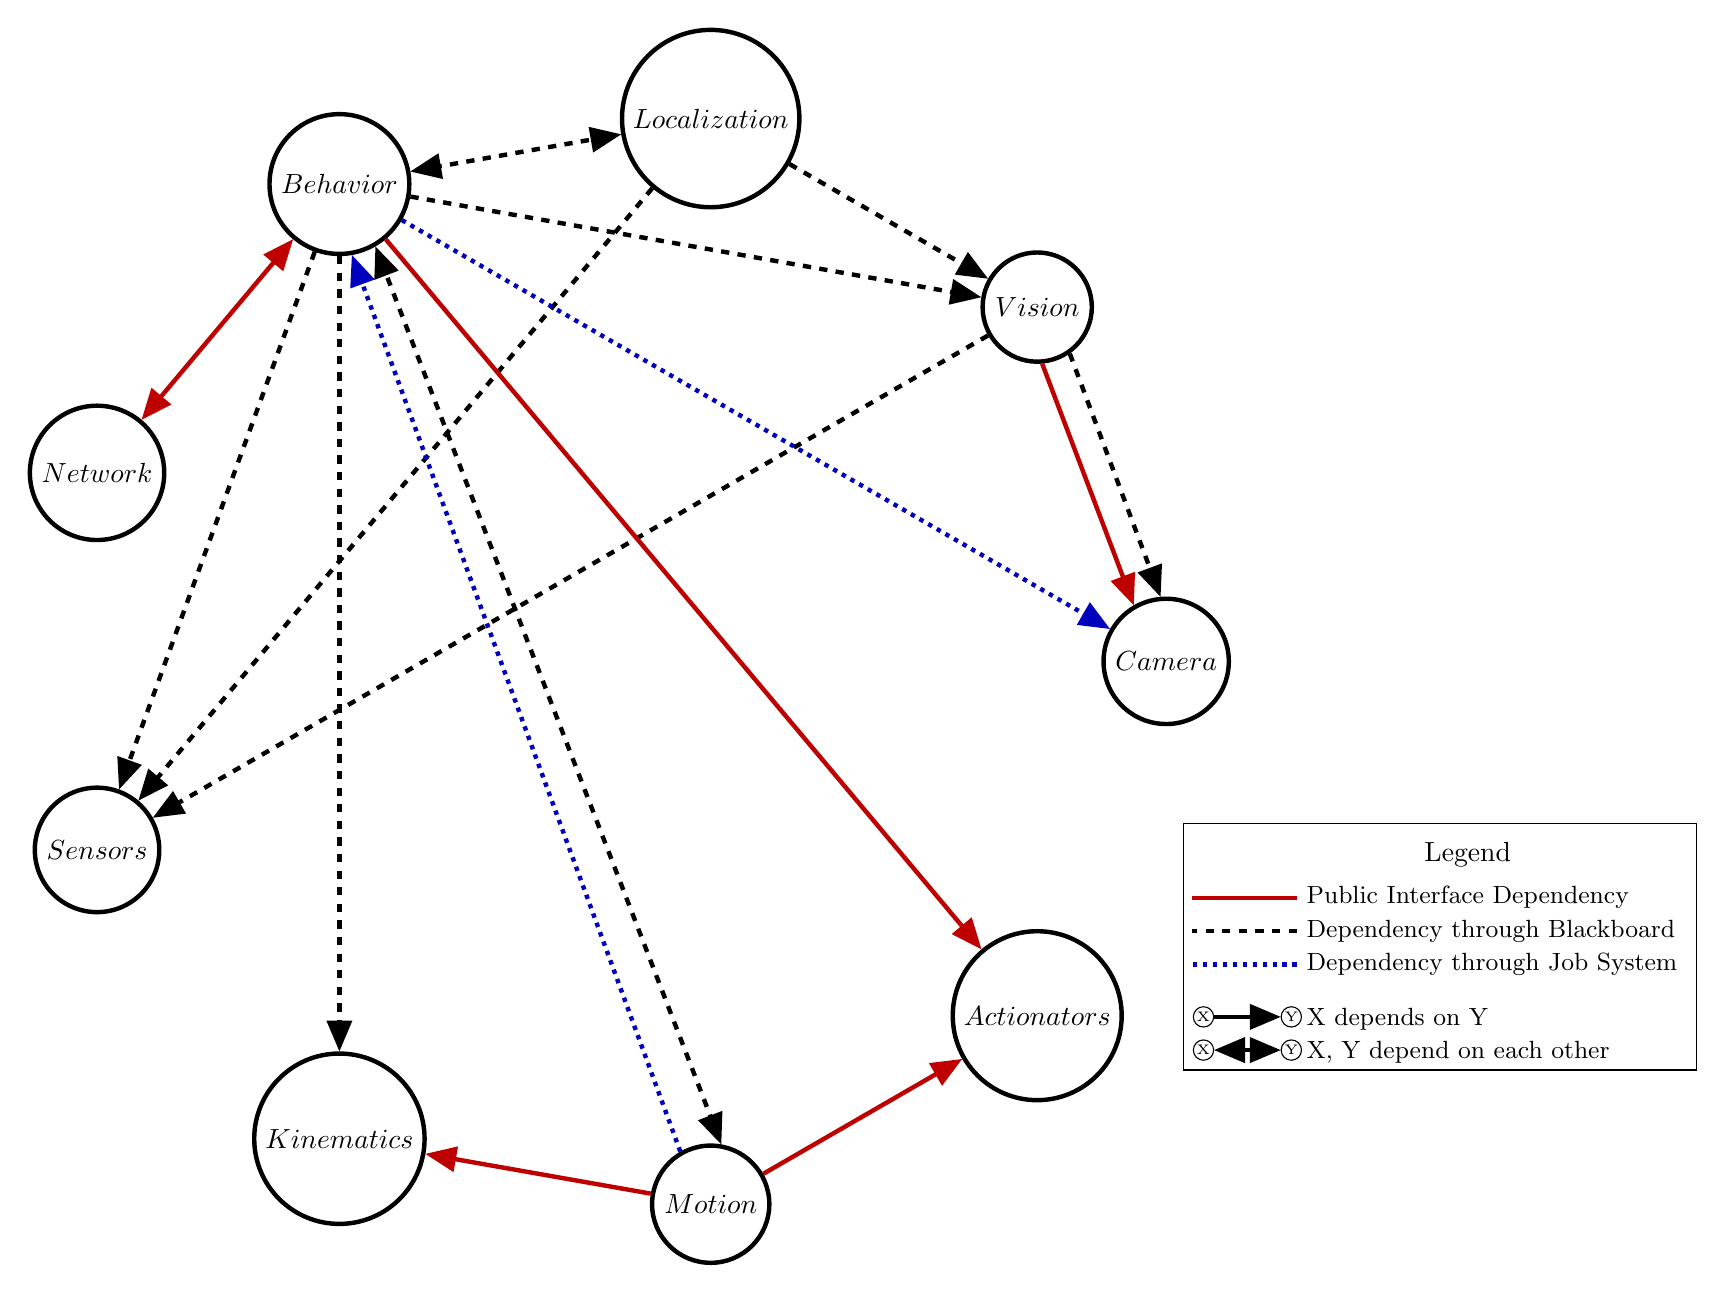
\begin{tikzpicture}[
		reactor/.style={draw, circle, ultra thick}
		, basearrow/.style={>=triangle 45, ultra thick}
		, blackboard/.style={basearrow, dashed}
		, publicinterface/.style={basearrow, color=red!75!black}
		, jobs/.style={basearrow, dotted, color=blue!75!black}
		, dependent/.style={->}
		, codependent/.style={<->}]

		%%% Legend
		\coordinate (legendpoint) at (13, -2);

		%% Public Interface Dependency
		\node [below=of legendpoint,anchor=east] (publicinterfacelabel) {\small Public Interface Dependency};
		\draw [publicinterface] (publicinterfacelabel.mid west) -- ++(-38pt, 0pt);

		%% Blackboard Dependency
		\node [below=12pt of publicinterfacelabel.south west,anchor=south west] (blackboardlabel) {\small Dependency through Blackboard};
		\draw[blackboard] (blackboardlabel.mid west) -- ++(-38pt, 0pt);

		%% Jobs Dependency
		\node [below=12pt of blackboardlabel.south west,anchor=south west] (joblabel) {\small Dependency through Job System};
		\draw[jobs] (joblabel.mid west) -- ++(-38pt, 0pt);

		%% Dependancy Type: Depends on
		\node[below=20pt of joblabel.south west,anchor=south west] (dependencylabel) {\small X depends on Y};
		\node[circle, draw, inner sep=0.5pt] (dependencynodeY) at ([yshift=1pt,xshift=-2pt]dependencylabel.mid west) {\tiny Y};
		\node[circle, draw, inner sep=0.5pt, left=24pt of dependencynodeY] (dependencynodeX) {\tiny X};
		\draw[basearrow, dependent] (dependencynodeX) edge (dependencynodeY);

		%% Dependancy Type: Codependent
		\node[below=12pt of dependencylabel.south west,anchor=south west] (codependencylabel) {\small X, Y depend on each other};
		\node[circle, draw, inner sep=0.5pt] (codependencynodeY) at ([yshift=1pt,xshift=-2pt]codependencylabel.mid west) {\tiny Y};
		\node[circle, draw, inner sep=0.5pt, left=24pt of codependencynodeY] (codependencynodeX) {\tiny X};
		\draw[basearrow, codependent] (codependencynodeX) edge (codependencynodeY);

		%% Legend Header
		\node[above=0pt of publicinterfacelabel] (legendheader) {Legend};

		%%% Draw all of our components in a circle
		\foreach [count=\i] \reactor in {Camera, Vision, Localization, Behavior, Network, Sensors, Kinematics, Motion, Actionators} {
		
			% Draw the reactors around the central star
			\node[reactor] (\reactor) at ({360/9 * (\i - 1)}:7cm) {$\reactor$};
		};

		%% Legend Border
		\node[fit=(legendheader)(publicinterfacelabel)(blackboardlabel)
				(joblabel)(dependencylabel)(codependencynodeX)(codependencynodeY),rectangle,draw](legendgroup){};

		%%% Dependencies
		%% Vision
		\path[blackboard, dependent] (Vision.305) edge (Camera.95);
		\path[publicinterface, dependent] (Vision.275) edge (Camera.120);
		\path[blackboard, dependent] (Vision) edge (Sensors);

		%% Localization
		\path[blackboard, dependent] (Localization) edge (Sensors);
		\path[blackboard, dependent] (Localization) edge (Vision);

		%% Behavior
		\path[blackboard, codependent] (Behavior) edge (Localization);
		\path[blackboard, dependent] (Behavior) edge (Kinematics);
		\path[blackboard, dependent] (Behavior) edge (Vision);
		\path[blackboard, dependent] (Behavior) edge (Sensors);
		\path[publicinterface, dependent] (Behavior) edge (Actionators);
		\path[publicinterface, codependent] (Behavior) edge (Network);
		\path[jobs, dependent] (Behavior) edge (Camera);

		%% Motion
		\path[blackboard, codependent] (Motion.80) edge (Behavior.300);
		\path[jobs, dependent] (Motion.120) edge (Behavior.280);
		\path[publicinterface, dependent] (Motion) edge  (Actionators);
		\path[publicinterface, dependent] (Motion) edge (Kinematics);
	\end{tikzpicture}
	\end{adjustbox}
\end{frame}

\begin{frame}
	\frametitle{Problems in Existing System}
	\begin{itemize}
		\item Hidden Dependencies
			\begin{itemize}
				\item The existing systems dependencies are very poorly defined
				\item For example, localizations dependency on the Stationary/Mobile object system.
				\item These hidden dependencies make it difficult to work on a system without understanding the whole system
			\end{itemize}
	
		\item Threading Issues
			\begin{itemize}
				\item Current system does not handle synchronisation between the two threads well
				\item e.g. The kick system can be prompted mid way by the walk engine, the two can even run together resulting in the robot standing still for prolonged periods.
				\item Happens because the interactions between the two threads is undefined in most cases
			\end{itemize}
	\end{itemize}
\end{frame}

\begin{frame}
	\frametitle{Problems in Existing System}
	\begin{itemize}			
		\item Network Communication
			\begin{itemize}
				\item Network communication is currently entirely through Localisation and Behaviour
				\item Adding new network communication requires modifying these two systems
				\item Because of the difficulty of adding new networking, no new networking will be added
			\end{itemize}
			
		\item Build System
			\begin{itemize}
				\item The current build system uses a make file that calls cmake that builds a make file that is called by the original make file
				\item This makes adding and removing components to the system in a meaningful way difficult
			\end{itemize}
	\end{itemize}
\end{frame}

\begin{frame}
	\frametitle{Wishlist}
	\begin{itemize}
		\item Modular Design
			\begin{itemize}
				\item Many modules that are made for robotics (walk engine, script engine) are useful for more then just soccer.
				\item Being able to use Mock inputs allows the system to be tested without access to a robot
				\item Being able to compose various modules into a binary would allow the robot to do more
				\item Enabling the sharing of these modules between researchers would result in better development (more people using the same code)
			\end{itemize}
			
		\item Transparent Multithreading
			\begin{itemize}
				\item Modern CPUs are getting more cores, rather then becoming faster
				\item Threading is difficult and can almost never be sensibly done at the module level
				\item Threading should be handled by the architecture in a way that can scale up to many cores
			\end{itemize}
	\end{itemize}
\end{frame}
			
\begin{frame}
	\frametitle{Wishlist}
	\begin{itemize}
		\item Runtime Statistics
			\begin{itemize}
				\item When optimising programs for speed it is useful to see how long each section of the code took
				\item Breaking up the modules and timing their execution better shows where CPU time is being used
			\end{itemize}
			
		\item Fine Grained Debugging
			\begin{itemize}
				\item When debugging a large system, there is often a low signal to noise ratio as a lot of debug lines are not useful
				\item Splitting up log lines based on source can help identify problems
				\item Being able to view the call graph in real time on a repeated process helps to identify links
			\end{itemize}
	\end{itemize}
\end{frame}

%----------------------------------------------------------------------------------------
\section{New Design}
%----------------------------------------------------------------------------------------
\begin{frame}
	\sectionpage
\end{frame}

\subsection{NUClear API}
\begin{frame}
	\frametitle{Software Architecture}
	\begin{itemize}
		\item If we are to replace the architecture of the existing system, we need to define what makes a good architecture
		\item A good software architecture is
		\begin{itemize}
			\item Maintainable
			\item Modifiable
			\item Testable
			\item Understandable
		\end{itemize}
	\end{itemize}
\end{frame}

\begin{frame}
	\frametitle{Coupling and Cohesion}
	\begin{itemize}
		\item The most powerful indicators for good architecture design are those of coupling and cohesion
		\item These two properties have huge influences on how easy a system is to understand and change
		\item A well designed system should be loosely coupled, and tightly cohesive
	\end{itemize}
\end{frame}

\begin{frame}
	\frametitle{Coupling}
	\begin{itemize}
		\item Coupling is a measure of how much a module relies on another module
		\item For example, if a module calls functions on another module, it is dependant on it
		\item A well designed system attempts to minimise these links between modules where possible
		\item It is also important to avoid irrelevant information being communicated
	\end{itemize}
\end{frame}

\begin{frame}
	\frametitle{Cohesion}
	\begin{itemize}
		\item Cohesion is a measure of the extent to which two elements of a single module belong together
		\item It describes the relevance of functionality within a module
		\item For example, if a single module contained only functionality for controlling a robots motion it would be tightly cohsevive
		\item However if a single module contained code for both performing vision processing as well as controlling the robots limbs this would be loosely cohesive as the two functions do not belong in a single logical module.
	\end{itemize}
\end{frame}

\begin{frame}
	\frametitle{Coupling}
	\begin{itemize}
		\item From an architectural standpoint, the decision of cohesion must be considered in each module
		\item However coupling must be designed for the entire architecture in order to ensure that communication between modules is loosely coupled
	\end{itemize}
\end{frame}

\begin{frame}
	\frametitle{Levels of Coupling}
	\begin{itemize}
		\item Coupling levels, from most coupled to least coupled are:
		\begin{itemize}
			\item Content Coupling (Pathological Coupling)
			\item Common Coupling (Global Coupling)
			\item External Coupling
			\item Control Coupling
			\item Stamp Coupling
			\item Data Coupling
			\item Message Coupling
			\item No Coupling
		\end{itemize}
		\item The existing architecture uses Common coupling through Blackboard (global storage)
	\end{itemize}
\end{frame}

\begin{frame}
	\frametitle{Message Passing}
	\begin{itemize}
		\item Message coupling is the least coupled method of communication
		\item Message passing systems have excellent maintainability and modifiability
		\item Components require no knowledge of each other
	\end{itemize}
\end{frame}

\begin{frame}
	\frametitle{Existing Systems}
	\begin{itemize}
		\item Message passing systems have been used in robotics before
		\item They have been used in most robotic architectures designed for large scale use
		\item These include
		\begin{itemize}
			\item Robot OS (ROS)
			\item Dynamic Data eXchange (DDX)
			\item CORBA based systems
		\end{itemize}
	\end{itemize}
\end{frame}

\begin{frame}
	\frametitle{Robot OS}
	\begin{itemize}
		\item ROS is of particular note as it is the most commonly used system used in research
		\item It currently runs in many robotic systems and has a substantial array of existing modules for it
		\item It is a distributed message passing system which allows multiple programming languages and machines
	\end{itemize}
\end{frame}

\begin{frame}
	\frametitle{Performance}
	\begin{itemize}
		\item These architectures are not suitable for use on the NUbots team robots
		\item They were designed to be used on high performance distributed systems
		\item The latency and processing overhead of the message passing is significant on slower systems
		\item This makes them unsuitable for lower performance devices such as the DARwIn-OP platform
	\end{itemize}
\end{frame}

\begin{frame}
	\frametitle{NUClear}
	\begin{itemize}
		\item To resolve these issues a new framework was designed named NUClear
		\item This framework and corresponding architecture is much faster then these previous systems
		\item This allows its use for the NUbots system
	\end{itemize}
\end{frame}

\begin{frame}
	\frametitle{NUClear Design}
	\centering
	\scalebox{0.55}{
		\begin{tikzpicture}[
				element/.style={
				circle,
				rounded corners,
				draw=black, very thick,
				minimum height=2em,
				text centered
			},
			arrow/.style={
				<->,
				thick
			},
			>=latex]
			
			\node [element] (plant) {PowerPlant};
		
			%%% Draw all of our components in a circle
			\foreach [count=\i] \reactor in {Reactor, Reactor, Reactor, Reactor, Reactor} {				
				% Draw the reactors around the central star
				\node [element] (reactor) at ({360/5 * (\i)}:6cm) {$\reactor$};
				
				\path [arrow] (plant) edge (reactor);
			};
			
		\end{tikzpicture}
	}
\end{frame}

\begin{frame}
	\frametitle{NUClear Design}
	\begin{itemize}
		\item NUClear is designed around a central PowerPlant
		\item The PowerPlant has several ``Reactors'' around it
		\item These reactors request data they need, and emit data they have created to it
		\item The PowerPlant will route this information to the appropriate entities
		\item The PowerPlant is also responsible for the storage of information
	\end{itemize}
\end{frame}

\begin{frame}
	\frametitle{NUClear Design}
	\begin{itemize}
		\item NUClear itself is built around the embedding of a Domain Specific Language (DSL) into C++
		\item It uses advanced C++ techniques in order to allow an intuitive description of data flow
		\item This allows it to be taught and used by novice C++ users while enforcing good practice
	\end{itemize}
\end{frame}

\begin{frame}
	\frametitle{Powerplant}
	\begin{itemize}
		\item The PowerPlant is the core component of the NUClear system
		\item It is the central point whereby communication between modules happens
		\item It holds the functionality to install modules and manages execution of the system
		\item Most of the time, you will users never directly interact with it (it is hidden)
	\end{itemize}
\end{frame}

\begin{frame}
	\frametitle{Reactor}
	\begin{itemize}
		\item A Reactor is the primary method that users will interact with the system
		\item It is a class that extends from NUClear::Reactor
		\item It has all of the methods on it that are used to listen for and emit messages
		\item They are installed these reactors into the PowerPlant
	\end{itemize}
\end{frame}

\begin{frame}
	\frametitle{Reaction}
	\begin{itemize}
		\item A reaction is a single function that is run in response to new data
		\item They take as arguments constant references to the data that they use
		\item The data that is passed into a reaction function can be considered thread safe
		\item The lifetime of the data used is managed by the PowerPlant
	\end{itemize}
\end{frame}

\begin{frame}
	\frametitle{NUClear Features}
	\begin{itemize}
		\item There have been several features integrated into NUClear which distinguish it as exceptional
		\item These include the following areas
		\begin{itemize}
			\item Transparent Multithreading
			\item Debugging Tools
			\item Integrated Networking
			\item Extensible API
		\end{itemize}
	\end{itemize}
\end{frame}

\begin{frame}
	\frametitle{Transparent Multithreading}
	\begin{itemize}
		\item NUClear is a multithreaded framework
		\item It will transparently multithread any code that is given to it
		\item This allows it to make use of all of the resources in the system
		\item This is also a significant advancement as it makes the system scaleable to future hardware
	\end{itemize}
\end{frame}

\begin{frame}
	\frametitle {Multi Threading}
	\begin{adjustbox}{max totalsize={\textwidth}{\textheight},center}
		\centering
		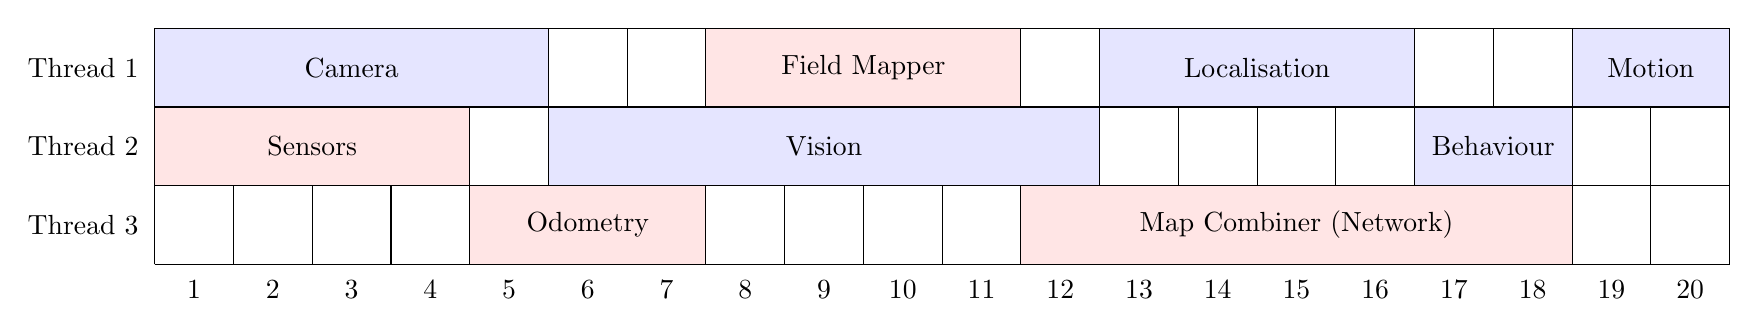
\begin{tikzpicture}
			\begin{scope}[
				task/.style={draw=black},
				cameratriggered/.style={fill=blue!10},
				sensortriggered/.style={fill=red!10}]

				\draw (1, 1) grid (21, 4);
				
				%% Thread 1
				\draw[cameratriggered, task] (1, 3) rectangle node {Camera} (6, 4);
				\draw[sensortriggered, task] (8, 3) rectangle node {Field Mapper} (12, 4);
				\draw[cameratriggered, task] (13, 3) rectangle node {Localisation} (17, 4);
				\draw[cameratriggered, task] (19, 3) rectangle node {Motion} (21, 4);
				
				%% Thread 2
				\draw[sensortriggered, task] (1, 2) rectangle node {Sensors} (5, 3);
				\draw[cameratriggered, task] (6, 2) rectangle node {Vision} (13, 3);
				\draw[cameratriggered, task] (17, 2) rectangle node {Behaviour} (19, 3);
				
				%% Thread 3
				\draw[sensortriggered, task] (5, 1) rectangle node {Odometry} (8, 2);
				\draw[sensortriggered, task] (12, 1) rectangle node {Map Combiner (Network)} (19, 2);
				
				% Row labels
				\node[anchor=east, inner sep=0] at (.8, 3.5) {Thread 1};
				\node[anchor=east, inner sep=0] at (.8, 2.5) {Thread 2};
				\node[anchor=east, inner sep=0] at (.8, 1.5) {Thread 3};
				
				% Column Labels
				\foreach \i in {1,...,20} {
				\node[anchor=north, inner sep=0] at (\i + .5, .8) {\i};
				}
			\end{scope}
		\end{tikzpicture}
	\end{adjustbox}
\end{frame}
\begin{frame}
	\frametitle{Debugging Tools}
	\begin{itemize}
		\item todo
	\end{itemize}
\end{frame}

\begin{frame}
	\frametitle{Integrated Networking}
	\begin{itemize}
		\item The networking system in NUClear is transparent to those using the system
		\item Any data can be sent over the network with no modification
		\item The syntax for emitting data over the network is identical to sending it to other modules
		\item This makes it trivial to perform network communication with other systems
	\end{itemize}
\end{frame}

\begin{frame}
	\frametitle{Networking}
	\begin{adjustbox}{max totalsize={\textwidth}{\textheight},center}
	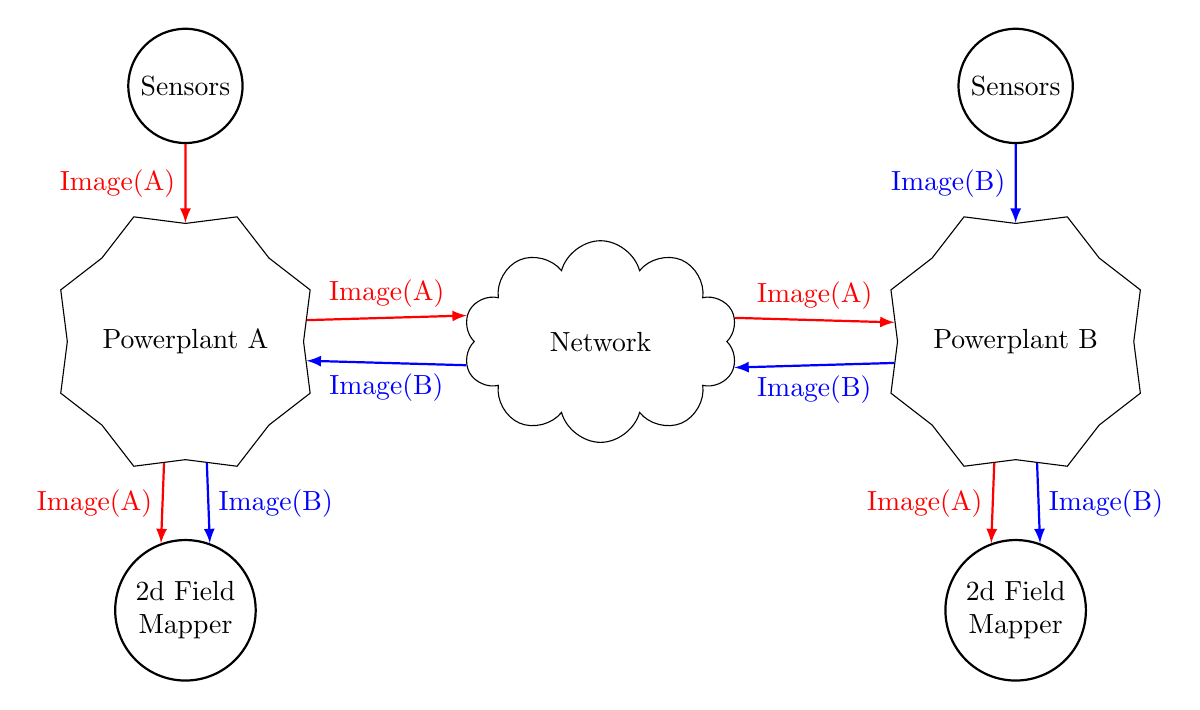
\begin{tikzpicture}[x=15em,y=5em,>=latex,
		A/.style={red},
		B/.style={blue},
		reactor/.style={draw, circle, thick},
		write/.style={->,thick},
		read/.style={<-,thick}]
	
		%%% Left Power Plant
		\node at (0, 0) [draw,star,star points=8,star point ratio=0.875,minimum width=3cm] (plantA) {Powerplant A};
		\node [above=of plantA,reactor] (sensorsA) {Sensors};
		\node [below=of plantA,reactor,align=center] (fieldmapperA) {2d Field\\Mapper};
		\path [A, write] (sensorsA) edge node[A,left] {Image(A)} (plantA);
		\path [A, read] (fieldmapperA.110) edge node[left] {Image(A)} (plantA.260);
		\path [B, read] (fieldmapperA.70) edge node[right] {Image(B)} (plantA.280);
	
		%%% Right Power Plant
		\node at (2, 0)
			[draw,star,star points=8,star point ratio=0.875,minimum width=3cm]
			(plantB){Powerplant B};
		\node [above=of plantB,reactor] (sensorsB) {Sensors};
		\node [below=of plantB,reactor,align=center] (fieldmapperB) {2d Field\\Mapper};
		\path [B, write] (sensorsB) edge node[left] {Image(B)} (plantB);
		\path [A, read] (fieldmapperB.110) edge node[left] {Image(A)} (plantB.260);
		\path [B, read] (fieldmapperB.70) edge node[right] {Image(B)} (plantB.280);
	
		%%% Network & Network Connections
		\node at (1, 0) [draw,cloud,cloud puffs=10,minimum width=3.5cm]
		(network) {Network};
	
		%% Plant A connections
		\path [A, write] (plantA.10) edge node[A, above] {Image(A)} (network.169);
		\path [B, read] (plantA.-9) edge node[B, below] {Image(B)} (network.190);
	
		%% Plant B connections
		\path [A, read] (plantB.171) edge node[A, above] {Image(A)}  (network.10);
		\path [B, write] (plantB.190) edge node[B, below] {Image(B)} (network.-11);
	\end{tikzpicture}
	\end{adjustbox}
\end{frame}

\begin{frame}
	\frametitle{Extensible API}
	\begin{itemize}
		\item The NUClear API itself was designed to be extensible
		\item The DSL which is defined in NUClear can be modified by the user
		\item This gives a lot of power to implement features within the language itself
		\item For example, the configuration system the the ported NUClear code is implemented as a part of the language
	\end{itemize}
\end{frame}

\begin{frame}
	\frametitle{Modular Design}
	\begin{itemize}
		\item The use of NUClear enforces modular design
		\item Every component must be placed in its own module
		\item Each module has a distinct purpose
	\end{itemize}
\end{frame}


%----------------------------------------------------------------------------------------
\subsection{NUClear Port}
%----------------------------------------------------------------------------------------
\begin{frame}
	\frametitle{NUClear Port}

	\begin{itemize}
		\item The NUbots software has been ported to use the NUClear architecture
		\item Functionality has been divided into many small, cohesive modules
		\item All communication across modules is accomplished through NUClear messages
		\item A new, flexible build system has been created with `roles' to allow fast and easy adding of functionality
	\end{itemize}
\end{frame}

\begin{frame}
	\frametitle{Modules}

	\begin{itemize}
		\item Every module has a single clear purpose, for example
		\begin{itemize}
			\item interacting with robot hardware
			\item running scripted movements
			\item loading configuration files
		\end{itemize}
		\item Modules do not care which other modules are present, only what information they consume and what they can produce
		\begin{itemize}
			\item Modules with the same inputs and outputs are interchangeable
			\item Platform details are inherently decoupled from everything else
		\end{itemize}
	\end{itemize}
\end{frame}

\begin{frame}
	\frametitle{Testing}

	\begin{itemize}
		\item Testing is built into the new system from the ground up
		\item Every module can have associated unit tests
		\item The build system can run unit tests as a batch
		\item It is easy to test single modules or subsets in isolation
		\item Can create testing modules that emulate input from hardware
	\end{itemize}
\end{frame}

\begin{frame}
	\frametitle{Orchestration}
	\begin{itemize}
		\item Thanks to modular design we can take inspiration from Service Oriented Architecture design
		\item Orchestration is the process of taking several modules and combining them to form an application
		\item The new build system uses `roles' to build behaviours from orchestrated modules
		\begin{itemize}
			\item Robocup role with soccer modules
			\item Marketing role for showing off the robots
			\item Script Tuner role with an interface for tweaking motion scripts
		\end{itemize}
		\item Many modules are shared by multiple roles
	\end{itemize}
\end{frame}

\begin{frame}
	\frametitle{Existing vs. New}
	
	\begin{itemize}
		\item In the existing system
		\begin{itemize}
			\item Inducting a new member into the project takes one month
			\item Changing behaviour requires detailed understanding, lots of code changes
		\end{itemize}
		\item In the NUClear port
		\begin{itemize}
			\item Modules are easy to learn and don't require understanding all their dependencies
			\item A new member can start doing useful work almost immediately
			\item Creating new roles requires changing only one file
		\end{itemize}
		\item `Mechwarrior' was created in under an hour on the new system, ``would have been impossible'' on the existing system
	\end{itemize}
\end{frame}


%----------------------------------------------------------------------------------------
\section{Robot Dance}
%----------------------------------------------------------------------------------------
	\begin{frame}
		\sectionpage %Title page for the Robot Dance section
	\end{frame}
	\subsection{What and Why?} %-------------------
	\begin{frame}
		\frametitle{Robot Dance: What and Why?}
		\begin{itemize}
			\item What does you mean by dancing robots?
			\begin{itemize}
				\item Scripted dancing
				\item Dancing in time with music
			\end{itemize}
			\item Why Dancing Robots?
			\begin{itemize}
				\item Demonstrates the efficiency of the new architecture
				\item Useful for marketing
			\end{itemize}
		\end{itemize}
	\end{frame}
	\subsection{Dancing to Music} %-------------------
	\begin{frame}
		\frametitle{Dancing to Music}
		\begin{itemize}
			\item Music detected through Microphone
			\item Music analysed to find beats
			\item Dance move chosen and scaled to be in time with latest beats
			\item Dance move is enacted
		\end{itemize}
	\end{frame}	
	\subsection{Dancing and NUClear} %-------------------
	\begin{frame}
		\frametitle{Dancing and the New Architecture}
		\framesubtitle{Dancing to a Music}
		\begin{figure}
			\centering
			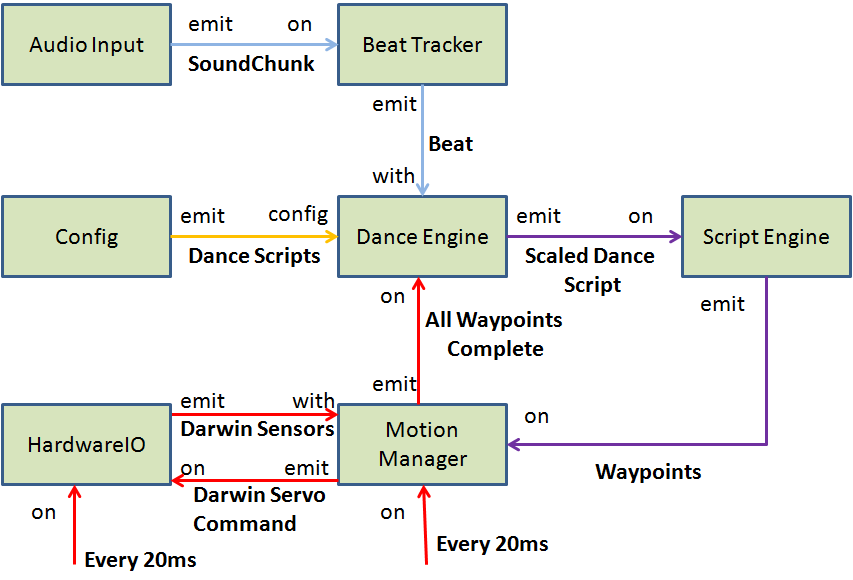
\includegraphics[scale=.45]{Presentation_Images/dance_audio_new_arc.png}
			\caption{Components for Dancing to Music with the NUClear}
		\end{figure}
	\end{frame}	
	\begin{frame}
		\frametitle{Dancing and the New Architecture}
		\framesubtitle{Dancing to a Music}
		\begin{figure}
			\centering
			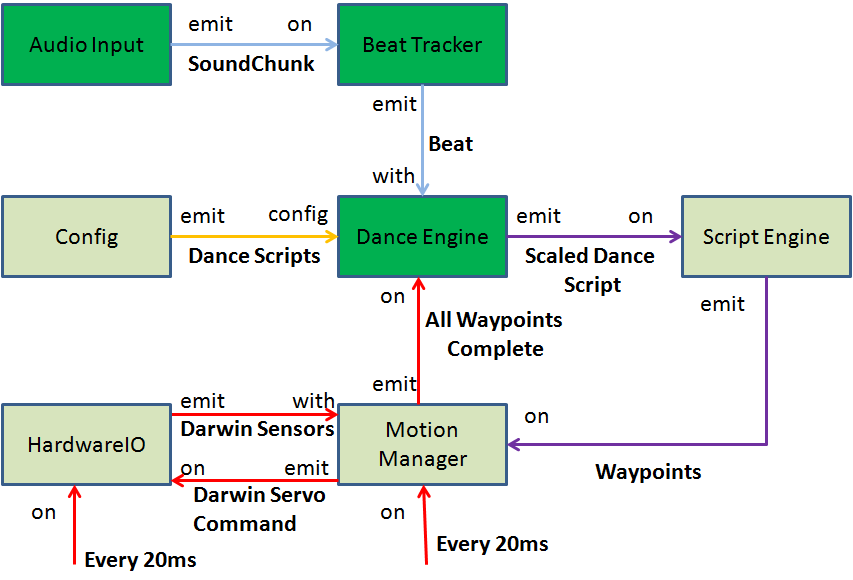
\includegraphics[scale=.45]{Presentation_Images/dance_audio_new_arc_change.png}
			\caption{Components for Dancing to Music with the NUClear}
		\end{figure}
	\end{frame}	
	\subsection{Dancing and the Old Architecture} %-------------------
	\begin{frame} %TODO update this picture
		\frametitle{Dancing and the Old Architecture}
		\framesubtitle{Dancing to a Music}
		\subimport{Presentation_Images/}{dance_audio_old_system.tex}
	\end{frame}	
	\begin{frame} %TODO get rid of this
		\frametitle{Dancing and the Old Architecture}
		\framesubtitle{Dancing to a Music}
		\begin{figure}
			\begin{adjustbox}{max totalsize={\textwidth}{.8\textheight},center}
			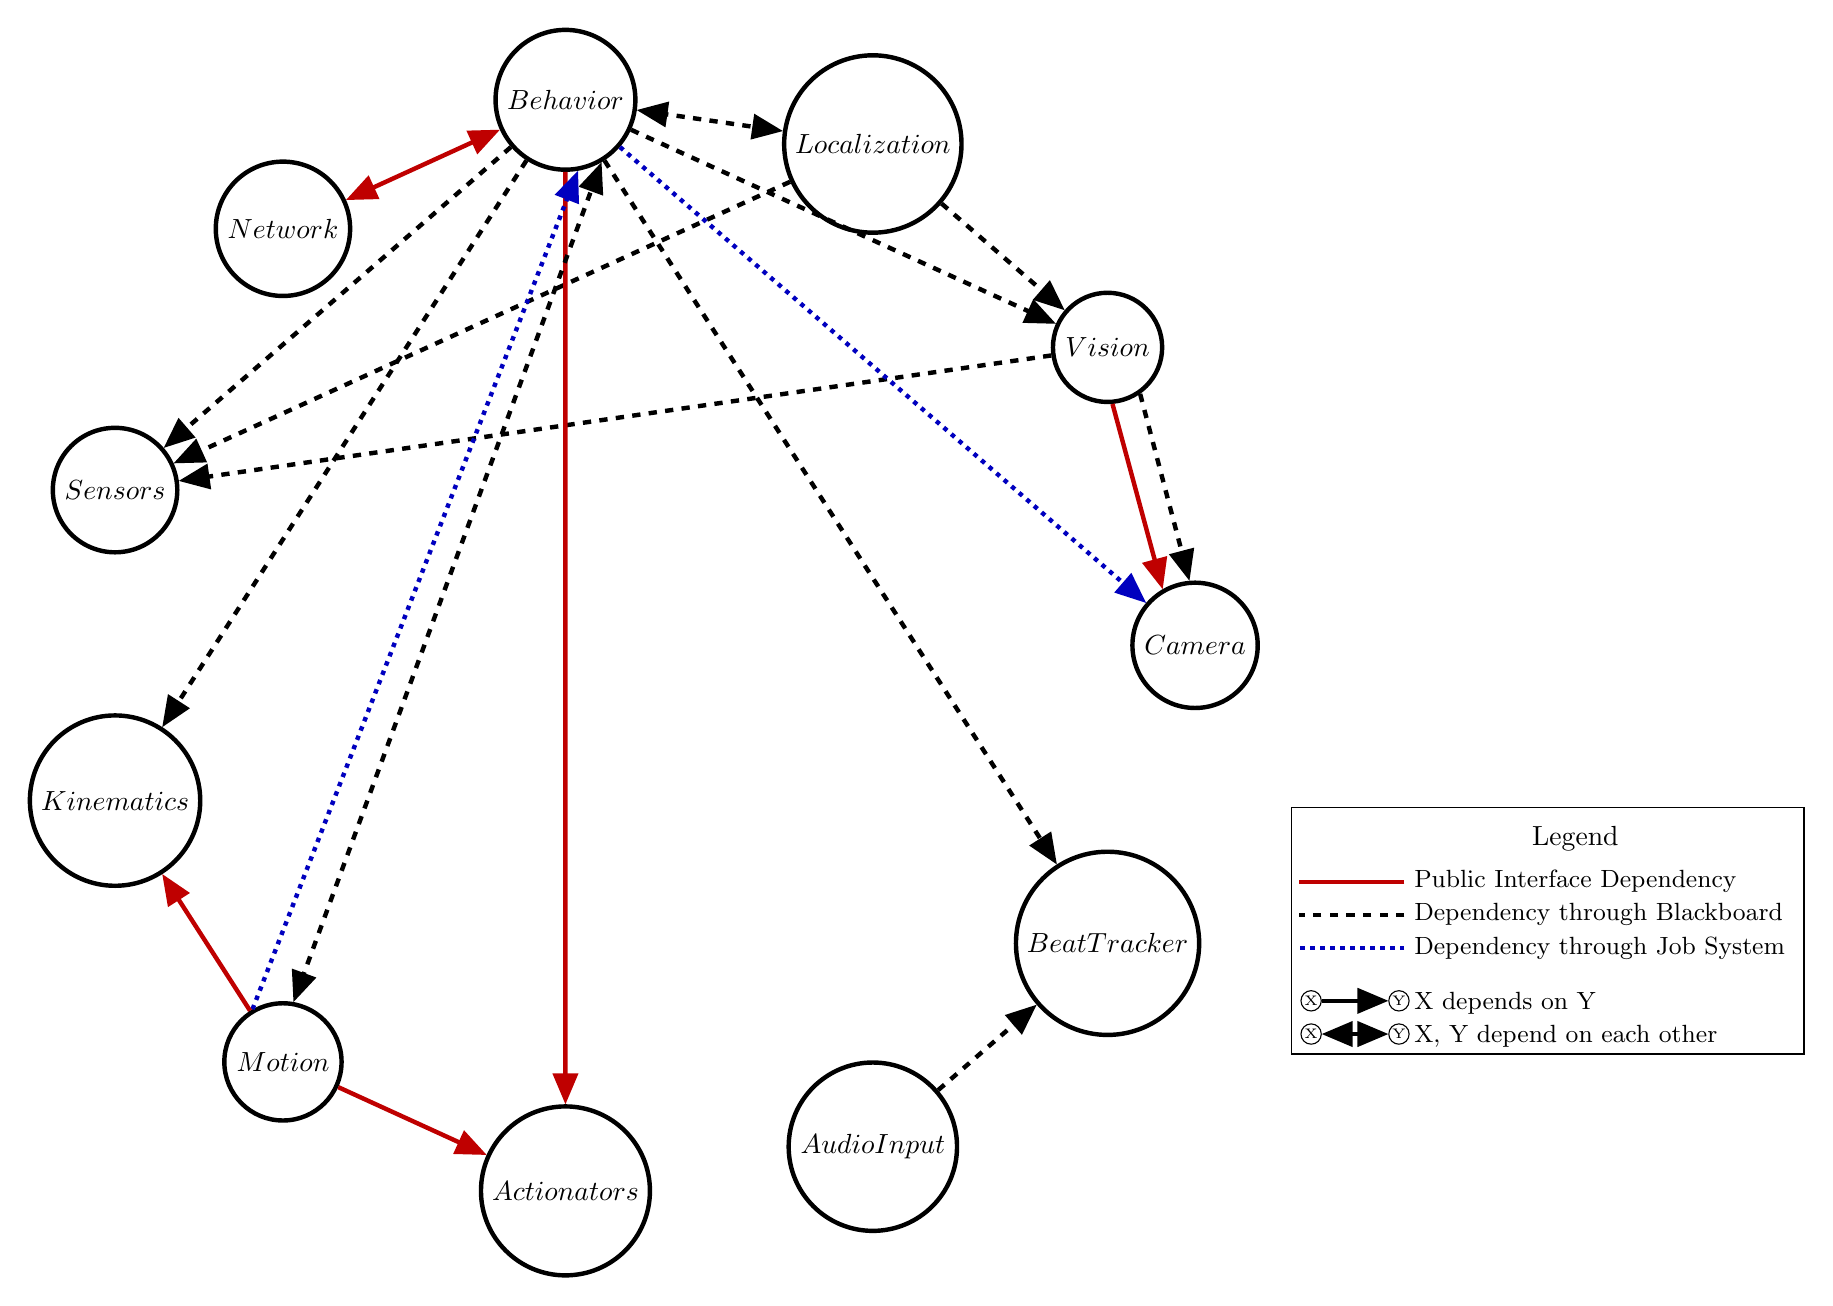
\begin{tikzpicture}[
				reactor/.style={draw, circle, ultra thick}
				, basearrow/.style={>=triangle 45, ultra thick}
				, blackboard/.style={basearrow, dashed}
				, publicinterface/.style={basearrow, color=red!75!black}
				, jobs/.style={basearrow, dotted, color=blue!75!black}
				, dependent/.style={->}
				, codependent/.style={<->}
				, new/.style={fill=green!45}
				, modified/.style={fill=green!75}]
		
				%%% Legend
				\coordinate (legendpoint) at (14, -2);
		
				%% Public Interface Dependency
				\node [below=of legendpoint,anchor=east] (publicinterfacelabel) {\small Public Interface Dependency};
				\draw [publicinterface] (publicinterfacelabel.mid west) -- ++(-38pt, 0pt);
		
				%% Blackboard Dependency
				\node [below=12pt of publicinterfacelabel.south west,anchor=south west] (blackboardlabel) {\small Dependency through Blackboard};
				\draw[blackboard] (blackboardlabel.mid west) -- ++(-38pt, 0pt);
		
				%% Jobs Dependency
				\node [below=12pt of blackboardlabel.south west,anchor=south west] (joblabel) {\small Dependency through Job System};
				\draw[jobs] (joblabel.mid west) -- ++(-38pt, 0pt);
		
				%% Dependancy Type: Depends on
				\node[below=20pt of joblabel.south west,anchor=south west] (dependencylabel) {\small X depends on Y};
				\node[circle, draw, inner sep=0.5pt] (dependencynodeY) at ([yshift=1pt,xshift=-2pt]dependencylabel.mid west) {\tiny Y};
				\node[circle, draw, inner sep=0.5pt, left=24pt of dependencynodeY] (dependencynodeX) {\tiny X};
				\draw[basearrow, dependent] (dependencynodeX) edge (dependencynodeY);
		
				%% Dependancy Type: Codependent
				\node[below=12pt of dependencylabel.south west,anchor=south west] (codependencylabel) {\small X, Y depend on each other};
				\node[circle, draw, inner sep=0.5pt] (codependencynodeY) at ([yshift=1pt,xshift=-2pt]codependencylabel.mid west) {\tiny Y};
				\node[circle, draw, inner sep=0.5pt, left=24pt of codependencynodeY] (codependencynodeX) {\tiny X};
				\draw[basearrow, codependent] (codependencynodeX) edge (codependencynodeY);
		
				%% Legend Header
				\node[above=0pt of publicinterfacelabel] (legendheader) {Legend};
		
				%%% Draw all of our components in a circle
				\foreach [count=\i] \reactor/\style in {Camera, Vision, Localization, {Behavior/modified}, Network, Sensors, Kinematics, {Motion/modified}, Actionators, {AudioInput/new}, {BeatTracker/new}} {
				
					% Draw the reactors around the central star
					\node[reactor] (\reactor) at ({360/11 * (\i - 1)}:7cm) {$\reactor$};
				};
		
				%% Legend Border
				\node[fit=(legendheader)(publicinterfacelabel)(blackboardlabel)
						(joblabel)(dependencylabel)(codependencynodeX)(codependencynodeY),rectangle,draw](legendgroup){};
		
				%%% Dependencies
				%% Vision
				\path[blackboard, dependent] (Vision.305) edge (Camera.95);
				\path[publicinterface, dependent] (Vision.275) edge (Camera.120);
				\path[blackboard, dependent] (Vision) edge (Sensors);
		
				%% Localization
				\path[blackboard, dependent] (Localization) edge (Sensors);
				\path[blackboard, dependent] (Localization) edge (Vision);
		
				%% Behavior
				\path[blackboard, codependent] (Behavior) edge (Localization);
				\path[blackboard, dependent] (Behavior) edge (Kinematics);
				\path[blackboard, dependent] (Behavior) edge (Vision);
				\path[blackboard, dependent] (Behavior) edge (Sensors);
				\path[publicinterface, dependent] (Behavior) edge (Actionators);
				\path[publicinterface, codependent] (Behavior) edge (Network);
				\path[jobs, dependent] (Behavior) edge (Camera);
		
				%% Motion
				\path[blackboard, codependent] (Motion.80) edge (Behavior.300);
				\path[jobs, dependent] (Motion.120) edge (Behavior.280);
				\path[publicinterface, dependent] (Motion) edge  (Actionators);
				\path[publicinterface, dependent] (Motion) edge (Kinematics);
				
				%% Dance
				\path[blackboard, dependent] (AudioInput) edge (BeatTracker);
				\path[blackboard, dependent] (Behavior) edge (BeatTracker);
			\end{tikzpicture}
			\end{adjustbox}

			\caption{Components for Dancing to Music with the Old System}
		\end{figure}
	\end{frame}	
	\subsection{Conclusions} %-------------------
	\begin{frame}
		\frametitle{Conclusions from Robot Dance}
			\begin{itemize}
				\item Robot Dance shows NUClear to be:
				\begin{itemize}
					\item Easy to learn
					\item Easy to use
					\item Modular
					\item Loosely Coupled
				\end{itemize}
			\end{itemize}
	\end{frame}	
	
\begin{frame}
% TODO conclusion and group reflection
\end{frame}

%----------------------------------------------------------------------------------------
\section{Individual Research}
%----------------------------------------------------------------------------------------
\begin{frame}
	\sectionpage
\end{frame}

	%----------------------------------------------------------------------------------------
	\subsection{Overcoming Limits of Event Driven Systems}
	%----------------------------------------------------------------------------------------
	\begin{frame}
		\subsectionpage
	\end{frame}
	
	%----------------------------------------------------------------------------------------
	\subsection{Compile Time Message Routing}
	%----------------------------------------------------------------------------------------
	\begin{frame}
		\subsectionpage
	\end{frame}
	
	\begin{frame}
		\frametitle{Software Architecture}
		\begin{itemize}
			\item Components in a well designed software architecture are:
			\item Loosely Coupled
			\item Tightly Cohesive
			\item These properties makes it easy to modify and maintain the system
		\end{itemize}
	\end{frame}
	
	\begin{frame}
		\frametitle{Message Passing}
		\begin{itemize}
			\item Message passing is the most loosely coupled architectural style
			\item Components do not need to know of each other at all
			\item This makes it easy to develop and modify components
		\end{itemize}
	\end{frame}
	
	\begin{frame}
		\frametitle{Use in Other Systems}
		\begin{itemize}
		\item Message passing has been used as an architecture with robotics before
			\item Robot OS (ROS) is based on a message passing architecture
			\item DDX is a previous generation robotics system also based on message passing
			\item CORBA is used extensively as a base for robotic systems
		\end{itemize}
	\end{frame}
	
	\begin{frame}
		\frametitle{Use in other Systems}
		\begin{itemize}
			\item These systems use message passing as it make it easy to collaborate and design modules
			\item However these systems were never designed to run on low powered hardware
			\item Robot OS for example was designed to run on multiple computers as a distributed application
			\item In order to do this it has heavy routing and serialisation requirements
		\end{itemize}
	\end{frame}
	
	\begin{frame}
		\frametitle{Metaprogramming}
		\begin{itemize}
			\item A Metaprogram is a programs that manipulate itself
			\item This includes programs that run at compilation time rather then runtime
			\item It allows work to be offloaded from runtime processing
		\end{itemize}
	\end{frame}
	
	\begin{frame}
		\frametitle{C++ Template Metaprogramming}
		\begin{itemize}
			\item C++ metaprogramming is done through templates
			\item Templates were designed to implement generic programming
			\item However they also accidentally as a side effect are a turing complete language
			\item This allows programs to be executed using templates at compile time using the type system
		\end{itemize}
	\end{frame}
		
	\begin{frame}
		\frametitle{Partial Evaluation}
		\begin{itemize}
			\item One such metaprogramming technique is partial evaluation
			\item It applies when partial information is available at compile time
			\item Partial evaluation takes a function and performs part of the evaluation during compilation
			\item In the case of a message passing system the routing of the message is known
		\end{itemize}
	\end{frame}
	
	\begin{frame}
		\frametitle{Compile Time Message Routing}
		\begin{itemize}
			\item We know the routes messages are going to take at compile time
			\item Messages are published subscribed to using types
			\item We can evaluate the dispatch of these messages at compile time using template metaprograms
			\item We can bind the data of the messages at runtime
		\end{itemize}
	\end{frame}
	
	\begin{frame}
		\frametitle{Before Compilation}
		\centering
		\scalebox{0.55}{
			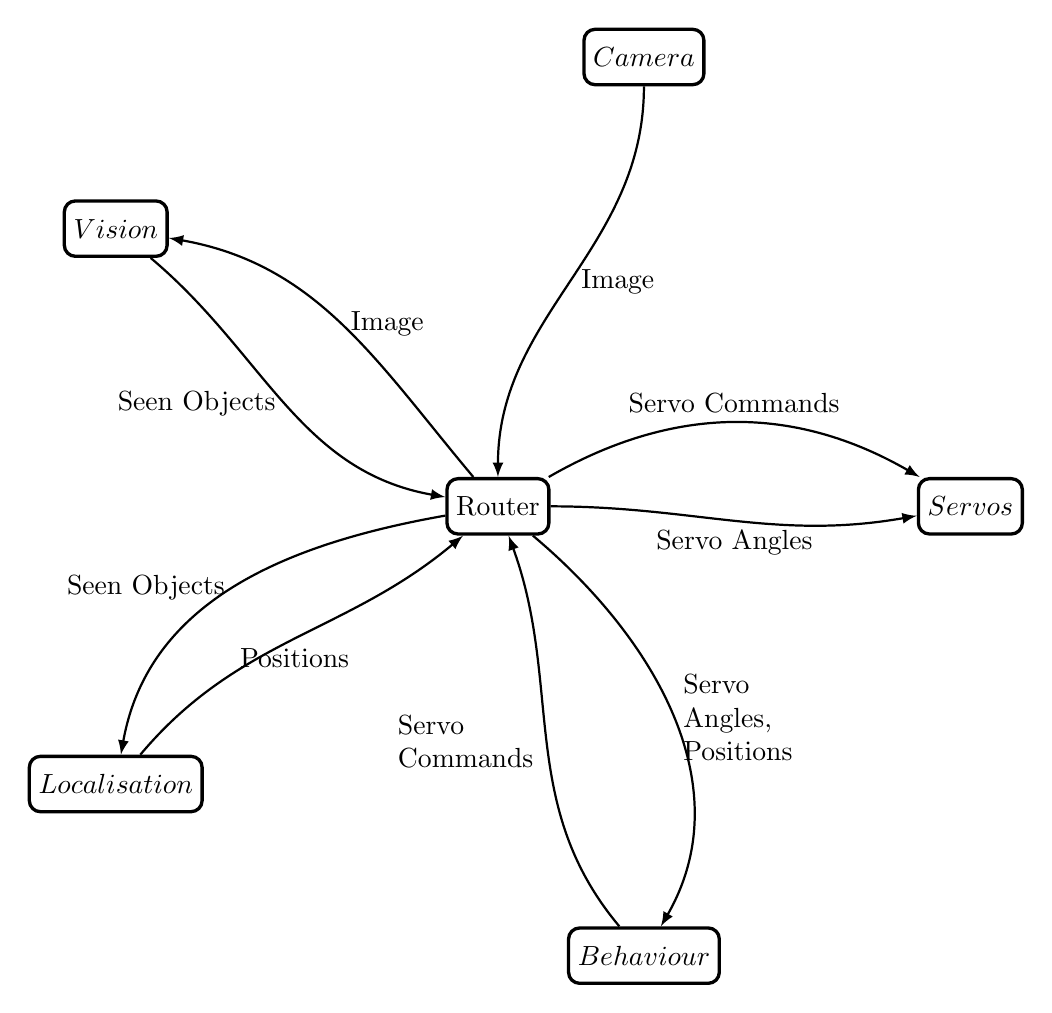
\begin{tikzpicture}[
				element/.style={
				rectangle,
				rounded corners,
				draw=black, very thick,
				minimum height=2em,
				text centered
			},
			ball/.style={
				element,
				minimum height=0,
				fill=black
			},
			arrow/.style={
				->,
				thick
			},
			>=latex]
			
			\node [element] (router) {Router};
		
			%%% Draw all of our components in a circle
			\foreach [count=\i] \reactor in {Camera, Vision, Localisation, Behaviour, Servos} {				
				% Draw the reactors around the central star
				\node [element] (msg\reactor) at ({360/5 * (\i)}:6cm) {$\reactor$};
			};
			
			\path [arrow] (router) edge[out=130, in=350]  node[right] {Image} (msgVision);
			\path [arrow] (msgVision) edge[out=320, in=170] node[left] {Seen Objects} (router);
			
			\path [arrow] (msgCamera) edge[out=270, in=90] node[right] {Image} (router);
			
			\path [arrow] (router) edge[out=320, in=60] node[right, text width=1.5cm] {Servo Angles, Positions} (msgBehaviour);
			\path [arrow] (msgBehaviour) edge[out=130, in=290] node[left, text width=1.75cm] {Servo Commands} (router);
			
			\path [arrow] (router) edge[out=190, in=80] node[left] {Seen Objects} (msgLocalisation);
			\path [arrow] (msgLocalisation) edge[out=50, in=220] node[below] {Positions} (router);
			
			\path [arrow] (router) edge[out=30, in=150] node[above] {Servo Commands} (msgServos);
			\path [arrow] (router) edge[out=0, in=190] node[below] {Servo Angles} (msgServos);
			
		\end{tikzpicture}}
	\end{frame}
	
	\begin{frame}
		\frametitle{After Compilation}
		\centering
		\scalebox{0.8}{
			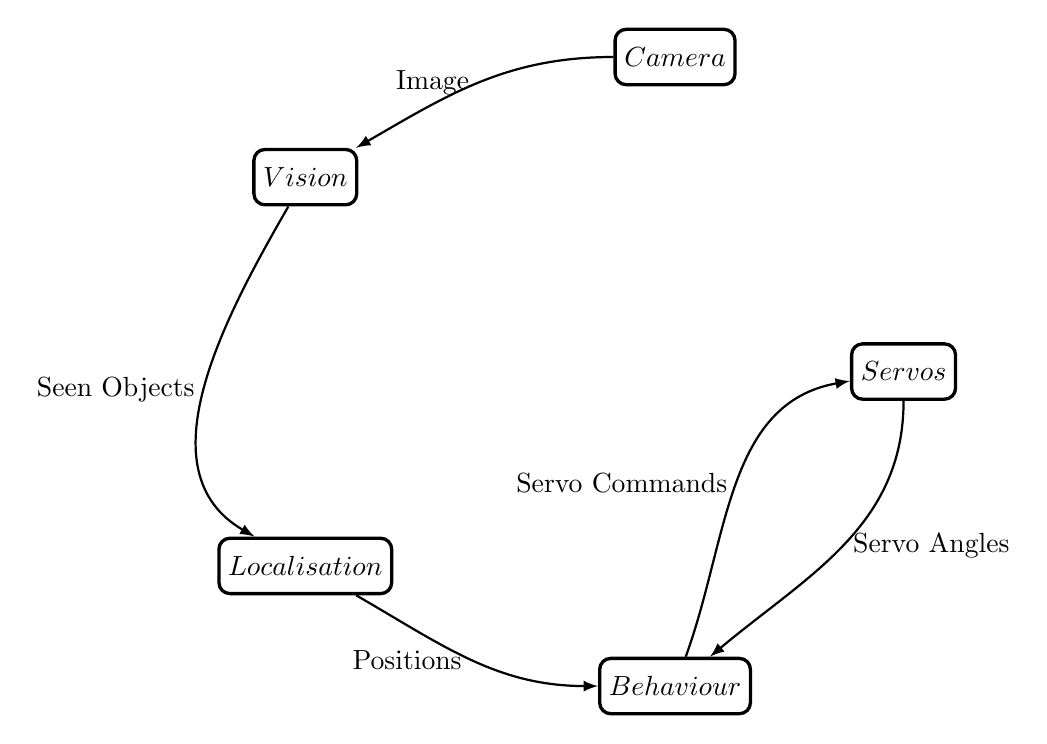
\begin{tikzpicture}[
				scale=0.7,
				element/.style={
					rectangle,
					rounded corners,
					draw=black, very thick,
					minimum height=2em,
					text centered
				},
				ball/.style={
					element,
					minimum height=0,
					fill=black
				},
				arrow/.style={
					->,
					thick
				},
				>=latex]
		
			%%% Draw all of our components in a circle
			\foreach [count=\i] \reactor in {Camera, Vision, Localisation, Behaviour, Servos} {				
				% Draw the reactors around the central star
				\node [element] (comp\reactor) at ({360/5 * (\i)}:6cm) {$\reactor$};
			}; 
			
			\path [arrow] (compCamera) edge[out=180, in=30] node[left] {Image} (compVision);
			\path [arrow] (compVision) edge[out=240, in=150] node[left] {Seen Objects} (compLocalisation);
			\path [arrow] (compLocalisation) edge[out=330, in=180] node[left] {Positions} (compBehaviour);
			\path [arrow] (compBehaviour) edge[out=70, in=190] node[left] {Servo Commands} (compServos);
			\path [arrow] (compServos) edge[out=270, in=40] node[right] {Servo Angles} (compBehaviour);
			
		\end{tikzpicture}}
	\end{frame}
	
	\begin{frame}
		\frametitle{Compile Time  Message Routing}
		\begin{itemize}
			\item Before compilation, every item only knows about the router
			\item This makes it very simple to modify programs
			\item After compilation components directly access each other
			\item This makes the resulting system almost as fast as direct function access
		\end{itemize}
	\end{frame}
	
	\begin{frame}
		\frametitle{Compile Time  Message Routing}
		\begin{itemize}
			\item The fast final result from the compile time program allows this architecture to be used
			\item The performance drawbacks of having a message router no longer apply
			\item This allows this style of architecture to be used in performance critical use cases
		\end{itemize}
	\end{frame}
	
	\begin{frame}
		\frametitle{Drawbacks}
		\begin{itemize}
			\item Using compile time message routing has drawbacks
			\item As the routing is performed at compile time, compilation of programs is slower
			\item Also, as template meta-programming in c++ is complex this makes it difficult to use
			\item It also results in larger binaries as the routes for messages are hard coded
			\item The system also requires an optimising compiler, else the system ends slower then a typical function call
		\end{itemize}
	\end{frame}
	
	\begin{frame}
		\frametitle{Results}
		\begin{itemize}
			\item When compared other methods of message passing compile time routing performed orders of magnitude faster
			\item As routing is performed at compile time, it also does not suffer from a slowdown as the number of publishers, subscribers, or message types increases
			\item The system was compared to CORBA for latency
			\item Compile time dispatch was measured as taking from the range of 300 nanoseconds to 1 microsecond
			\item CORBA is measured as taking between 1 millisecond to 7 milliseconds
		\end{itemize}
	\end{frame}
	
	\begin{frame}
		\frametitle{Use in FYP}
		\begin{itemize}
			\item Compile time message routing is used within the NUClear framework in order to route messages
			\item This allows it to perform orders of magnitude faster then competing architectures
			\item It also does not suffer slowdowns with the size of the project
		\end{itemize}
	\end{frame}
	
	%----------------------------------------------------------------------------------------
	\subsection{Efficient Multithreading in Message Passing Systems}
	%----------------------------------------------------------------------------------------
	\begin{frame}
		\subsectionpage
	\end{frame}
	
	%----------------------------------------------------------------------------------------
	\subsection{Beat Tracking}
	%----------------------------------------------------------------------------------------
	\begin{frame}
		\subsectionpage
	\end{frame}
	\begin{frame}
		Can Beat Tracking accurately detect beats in real time for Robot Dance?
	\end{frame}
	\begin{frame}
		What is beat tracking?
		\begin{itemize}
			\item Beat is the basic timing element of music
			\item Beats occur at regular intervals
			\item Tapping along to music is beat tracking
			\item Software beat trackers analyse audio input to find the locations of beats.
		\end{itemize}
	\end{frame}
	\begin{frame}
		How a software beat tracker could work
		\begin{itemize}
			\item Onset detection used to find location of musical notes in audio
			\item Notes that occur at regular intervals are found
			\item The most prominent regular notes are taken to be the beat
		\end{itemize}
	\end{frame}
	\begin{frame}
		Criteria for the Beat Tracker:
		\begin{itemize}
			\item Real Time % Whole piece of music doesn't need to be analysed. Works with microphone input.
			\item Quick % Doesn't slow down other systems. Beat found before the next beat occurs.
			\item Accurate % Beats found are close enough to where a listener feels they should be
			\item Robust	% Works in real audio situations with background noise an Robot motor noise.		
		\end{itemize}
	\end{frame}
	\begin{frame}
		Real Time:
		\begin{itemize}
			\item Does not require analysing the whole song to find the beats
			\item Uses past events to find beats but not future events.
			\item Can take in audio through microphone and analyse incrementally
		\end{itemize}		
	\end{frame}
	\begin{frame}
		Quick:
		\begin{itemize}
			\item Doesn't slow down the rest of the system.
			\item Beat located before next audio containing a beat is input into system
		\end{itemize}		
	\end{frame}
	\begin{frame}
		Accurate:
		\begin{itemize}
			\item Measures highly on beat tracker evaluation tests
			\item Beats found feel right to a listener.
			\item Accuracy doesn't need to be perfect
			\begin{itemize}
				\item Can't be perfectly on the beat
				\item Half-pace beats may still feel right to a user
			\end{itemize}	
		\end{itemize}		
	\end{frame}
	\begin{frame}
		Robust:
		\begin{itemize}
			\item Works in real audio situations
			\item Able to ignore background noise
			\item Biggest problem for robots is motor noise
		\end{itemize}		
	\end{frame}
	\begin{frame}
		Two Candidates:
		\begin{itemize}
			\item Aubio
				\begin{itemize}
					\item Not the most accurate but it is quick
				\end{itemize}
			\item Beat'n
				\begin{itemize}
					\item Beat tracker Trent wrote when we were trying to get Aubio to work
				\end{itemize}
		\end{itemize}		
	\end{frame}
	\begin{frame}
		Testing the 2 Beat Trackers for accuracy:
		\begin{itemize}
			\item Tested on 20, thirty second snippets of music
			\item Compared results of Beat Trackers with beats found by a human
			\item Comparisons evaluated by 6 evaluation methods (some with several variations)
			\item In addition to testing Aubio and Beat'n, we also test a dummy algorithm which simply has a beat occur every 0.5 seconds
		\end{itemize}		
	\end{frame}
%	\begin{frame}
%		Testing results:
%		\begin{table}
%		\begin{tabular}{c c c c c c c c c c c}
%			          & F-Measure & Cem(acc) & Goto(acc) & P-Score & CMLc & CMLt & AMLc & AMLt & D & Dg \\
%			Aubio & 29.6205 & 20.9227 & 0 & 35.5261 & 9.3504 & 14.2556 & 20.0702 & 31.6623 & 0.9857 & 0.0723 \\
%			Beat'n & 22.8261 & 15.7258 & 0 & 28.6636 & 3.054 & 5.8672 & 17.6479 & 25.7328 & 0.9178 & 0.0527 \\
%			Dummy & 8.227 & 5.7759 & 0 & 7.0067 & 0.7358 & 1.6722 & 1.5552 & 3.3445 & 0.0253 & 0.0083 \\
%		\end{tabular}
%		\end{table}	
%	\end{frame}
	\begin{frame}
		Testing results:
		\begin{table}
		\begin{tabular}{c | c | c | c }
			  & Aubio  & Beat'n  & Dummy\\ \hline
			F-Measure  & 29.62  & 22.83  & 27.93\\ \cline{1-1}  \cdashline{2-4}
			Cem(acc)  & 20.92  & 15.73  & 19.61\\ \cline{1-1}  \cdashline{2-4}
			Goto(acc)  & 0  & 0  & 0\\ \cline{1-1}  \cdashline{2-4}
			P-Score  & 35.53  & 28.66  & 36.91\\ \cline{1-1}  \cdashline{2-4}
			CMLc  & 9.35  & 3.05  & 4.16\\ \cline{1-1}  \cdashline{2-4}
			CMLt  & 14.26  & 5.87  & 9.37\\ \cline{1-1}  \cdashline{2-4}
			AMLc  & 20.07  & 17.65  & 8.87\\ \cline{1-1}  \cdashline{2-4}
			AMLt  & 31.66  & 25.73  & 19.07\\ \cline{1-1}  \cdashline{2-4}
			D  & 0.99  & 0.92  & 0.59\\ \cline{1-1}  \cdashline{2-4}
			Dg  & 0.0723  & 0.0527  & 0.0315\\ \cline{1-1}  \cdashline{2-4}
		\end{tabular}
		\end{table}	
	\end{frame}
	\begin{frame}
		Further testing for Aubio:
		\begin{itemize}
			\item Tested on 14 songs
			\item Compared with more modern beat trackers
		\end{itemize}		
	\end{frame}
	\begin{frame}
		Testing results:
		\begin{table}
		\begin{tabular}{c | c | c | c | c | c | c}
			& Davies & Kea & Dixon & Ellis & Dummy & Aubio \\ \hline
			F-Measure & 82.16 & 87.56 & 91.93 & 79.78 & 27.65 & 25.36 \\ \cline{1-1}  \cdashline{2-7}
			Cem(acc)  & 80.75 & 73.72 & 86.14 & 52.08 & 19.41 & 18.42 \\ \cline{1-1}  \cdashline{2-7}
			Goto(acc)  & 100 & 78.57 & 85.71 & 35.71 & 0 & 7.14 \\ \cline{1-1}  \cdashline{2-7}
			P-Score &  79.94 & 82.49 & 90.29 & 72.07 & 35.38 & 35.05 \\ \cline{1-1}  \cdashline{2-7}
			CMLc  & 76.45 & 58.68 & 76.62 & 37.17 & 4.54 & 7.82 \\ \cline{1-1}  \cdashline{2-7}
			CMLt  & 77.94 & 68.82 & 84.04 & 48.2 & 18.63 & 21.51 \\ \cline{1-1}  \cdashline{2-7}
			AMLc  & 77.26 & 79.95 & 79.84 & 39.72 & 4.93 & 16.12 \\ \cline{1-1}  \cdashline{2-7}
			AMLt  & 78.72 & 90.09 & 90.98 & 77.58 & 19.81 & 36.75 \\ \cline{1-1}  \cdashline{2-7}
			D  & 3.28 & 2.4 & 2.74 & 2.64 & 0.095 & 0.45 \\ \cline{1-1}  \cdashline{2-7}
			Dg  & 2.85 & 1.85 & 2.36 & 1.63 & 0.013 & 0.023 \\ \cline{1-1}  \cdashline{2-7}
		\end{tabular}
		\end{table}	
	\end{frame}
	\begin{frame}
		Difficulties with testing:
		\begin{itemize}
			\item Acquiring music with annotated beat locations
			\item Offbeats counted as completely wrong
			\item Dummy algorithm can score high, but conveys no information
		\end{itemize}
	\end{frame}
	\begin{frame}
		Evaluating the other criteria:
		\begin{itemize}
			\item Both algorithms work in real time
			\item Both algorithms are quick
			\item Aubio has big problems with Motor Noise, though a filter could fix it.
			\item Beat'n handle motor noise much better, though it still has some problem with it
		\end{itemize}
	\end{frame}
	\begin{frame}
		Conclusion:
		\begin{itemize}
			\item Beat Tracking CAN accurately detect beats in real time for Robot Dance
			\item Aubio and Beat'n are a little lacking but sufficient for the job
			\item Better beat trackers are available, particularly when more processing power is available.
		\end{itemize}
	\end{frame}
	\begin{frame}
		Core Papers:
		
	\end{frame}
	
\end{document} 
